% Diagram for the proof that "f is continuous iff preimage of every
% open set is open". Two metric spaces M (left) and N (right). On the
% right, an open set V containing a point y, with a small ε-ball
% inside V. On the left, the preimage U = f^pre(V), with a δ-ball
% around x ∈ U mapping into the ε-ball. Arrow f from M to N.
% Source: book/tex/topology/metric-top.tex (§ Open sets, theorem proof).
\documentclass[border=2mm]{standalone}
\usepackage{tikz}
\usetikzlibrary{calc}
\begin{document}
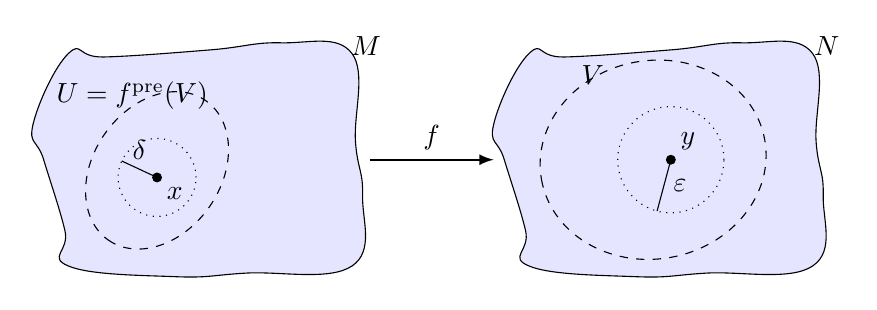
\begin{tikzpicture}[>=latex, scale=0.45]
  % --- Left: M with U = f^pre(V), x, δ-ball ---
  \begin{scope}
    \draw[fill=blue!10] plot[smooth cycle, tension=0.7] coordinates
      {(-4,3) (-5,1) (-4.7,0) (-4.1,-2) (-4,-3) (-1,-3.3) (1,-3.2)
       (4,-3) (4.3,-1) (4.1,0.5) (4,3) (2,3.3) (0,3.1) (-3,2.9)};
    \node at (4.4,3.2) {$M$};
    % U: dashed irregular region (rotated/scaled ellipse).
    \draw[dashed, rotate around={235:(-1.5,-0.3)},
          shift={(-1.5,-0.3)}] (0,0) ellipse (2.4 and 1.8);
    \node at (-2.2,1.8) {$U = f^{\mathrm{pre}}(V)$};
    % Point x and its δ-neighborhood.
    \fill (-1.5,-0.5) circle (4pt);
    \node[below right] at (-1.5,-0.5) {$x$};
    \draw[dotted] (-1.5,-0.5) circle (1.1);
    \draw (-1.5,-0.5) --
      ($(-1.5,-0.5) + ({1.1*cos(155)},{1.1*sin(155)})$);
    \node[above]
      at ($(-1.5,-0.5) + ({0.55*cos(155)},{0.55*sin(155)})$)
      {$\delta$};
  \end{scope}
  % --- Arrow f: M → N ---
  \draw[->, thick] (4.5,0) -- (8,0);
  \node[above] at (6.25,0) {$f$};
  % --- Right: N with V, y, ε-ball ---
  \begin{scope}[shift={(13,0)}]
    \draw[fill=blue!10] plot[smooth cycle, tension=0.7] coordinates
      {(-4,3) (-5,1) (-4.7,0) (-4.1,-2) (-4,-3) (-1,-3.3) (1,-3.2)
       (4,-3) (4.3,-1) (4.1,0.5) (4,3) (2,3.3) (0,3.1) (-3,2.9)};
    \node at (4.4,3.2) {$N$};
    % V: dashed irregular region (rotated/scaled ellipse).
    \draw[dashed, rotate around={190:(-0.5,0)}, shift={(-0.5,0)}]
      (0,0) ellipse (3.2 and 2.8);
    \node at (-2.2,2.4) {$V$};
    % Point y and its ε-neighborhood.
    \fill (0,0) circle (4pt);
    \node[above right] at (0,0) {$y$};
    \draw[dotted] (0,0) circle (1.5);
    \draw (0,0) -- ({1.5*cos(255)},{1.5*sin(255)});
    \node[right]
      at ({0.75*cos(255)},{0.75*sin(255)})
      {$\varepsilon$};
  \end{scope}
\end{tikzpicture}
\end{document}
